\subsection{UC18 - Cancellazione prodotto}
\begin{figure}[H]
  \centering
  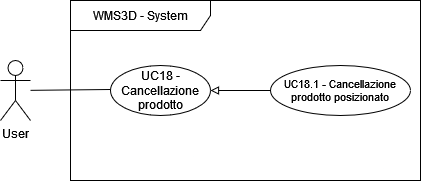
\includegraphics[width=0.8\textwidth]{UC_diagrams_11-20/UC18_sys.drawio.png}
   \caption{Diagramma UML UC18 - Cancellazione prodotto}
\end{figure}
\begin{figure}[H]
  \centering
  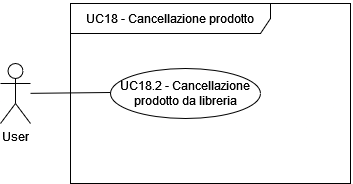
\includegraphics[width=0.8\textwidth]{UC_diagrams_11-20/UC18.drawio.png}
   \caption{Diagramma UML in dettaglio UC18 - Cancellazione prodotto}
\end{figure}
\begin{itemize}
    \item \textbf{Attori:} User.
    \item \textbf{Pre-condizione:} L'utente ha selezionato un prodotto [UC15].
    \item \textbf{Post-condizione:} Il prodotto viene eliminato dalla libreria e dal render 3D.
    \item \textbf{Scenario Principale:} L'utente elimina da libreria [UC18.2] il prodotto precedentemente selezionato. Se il prodotto era stato posizionato [UC18.1], lo elimina anche dal render 3D [UC18.1.1].
    \item \textbf{Generalizzazioni:} È presente una generalizzazione in caso in cui il prodotto sia stato posizionato:
    \begin{itemize}
        \item UC18.1 - Cancellazione prodotto posizionato.
    \end{itemize}
    \item \textbf{Estensioni:} -
\end{itemize}


\subsubsection{UC18.1 - Cancellazione prodotto posizionato}
\begin{figure}[H]
  \centering
  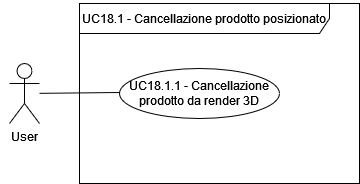
\includegraphics[width=0.8\textwidth]{UC_diagrams_11-20/UC18.1.drawio.png}
   \caption{Diagramma UML UC18.1 - Cancellazione prodotto posizionato}
\end{figure}
\begin{itemize}
    \item \textbf{Attori:} User.
    \item \textbf{Pre-condizione:} L'utente ha selezionato un prodotto [UC15] che è stato posizionato [UC14] e lo vuole eliminare.
    \item \textbf{Post-condizione:} L'utente elimina il prodotto dalla libreria e dal render 3D.
    \item \textbf{Scenario Principale:} L'utente elimina dalla libreria [UC18.2] e dal render 3D [UC18.1.1] il prodotto precedentemente selezionato.   
    \item \textbf{Generalizzazioni:} -
    \item \textbf{Estensioni:} -
\end{itemize}


\paragraph{UC18.1.1 - Cancellazione prodotto da render 3D}
\begin{itemize}
    \item \textbf{Attori:} User.
    \item \textbf{Pre-condizione:} L'utente ha selezionato un prodotto [UC15] che è stato posizionato [UC14] e lo vuole eliminare.
    \item \textbf{Post-condizione:} L'utente elimina il prodotto dal render 3D.
    \item \textbf{Scenario Principale:} L'utente elimina dal render 3D il prodotto posizionato precedentemente selezionato.   
    \item \textbf{Generalizzazioni:} -
    \item \textbf{Estensioni:} -
\end{itemize}


\subsubsection{UC18.2 - Cancellazione prodotto da libreria}
\begin{itemize}
    \item \textbf{Attori:} User.
    \item \textbf{Pre-condizione:} L'utente ha selezionato un prodotto [UC15] e lo vuole eliminare.
    \item \textbf{Post-condizione:} L'utente elimina il prodotto dalla libreria.
    \item \textbf{Scenario Principale:} L'utente elimina da libreria il prodotto precedentemente selezionato.   
    \item \textbf{Generalizzazioni:} -
    \item \textbf{Estensioni:} -
\end{itemize}